%\documentclass[twocolumn]{aastex62}
\documentclass[apj,iop]{emulateapj}
%\documentstyle[11pt,aas_macros]{article}
\usepackage{graphicx}
%\usepackage{subcaption}
\usepackage{subfigure}
\usepackage{amssymb,amsmath}
\usepackage{natbib}
\usepackage{gensymb}
%\bibliographystyle{aasjournal.bst}
\bibliographystyle{apj}
%\bibliographystyle{plainnat}
\usepackage{epsfig}
\setcitestyle{notesep={; }} %changes "," to ";" in Lang (2014, hereafter L14)
%\renewcommand{\thefootnote}{\fnsymbol{footnote}}
%\graphicspath{{./allfigures/}}

\begin{document}

%\title{Optical-faint, Far-infrared-bright {\textit{\textbf Herschel}} Sources
%in the CANDELS Fields: Ultra-Luminous Infrared Galaxies at \boldmath$z>1$ and
%the Effect of Source Blending
%\footnotemark[$\star$]}\footnotetext[$\star$]{Herschel is an ESA space 
%observatory with science instruments provided by European-led Principal
%Investigator consortia and with important participation from NASA.}

\title{Title
}
\author{Marat Musin \altaffilmark{1} \altaffilmark{2}, 
Haojing Yan \altaffilmark{2}, 
}

\altaffiltext{1}{Chinese Academy of Sciences South America Center for Astronomy
(CASSACA), National Astronomical Observatories, Chinese Academy of
Sciences, Beijing 100012, China}
\altaffiltext{2}{Department of Physics \& Astronomy, University of Missouri,
Columbia, MO 65211, USA}



\begin{abstract}

%\lipsum

\end{abstract}

\keywords{
 infrared: galaxies --- submillimeter: galaxies ---  galaxies: starburst ---
 methods: data analysis
}

\section{Introduction}

\subsection{Lilly-Madau formalism}

\subsection{SED fitting as a standard technique of mass and redshift estimation}
SED fitting is now a standard technique of deriving stellar mass and photometric redshifts for a large set of galaxies. In this method multi-band photometry for a given galaxy is fitted to a series of a templates predicted by a certain stellar population synthesis (SPS) model. The best-fit template gives the parameters of the galaxy, including its redshift and mass.
Historically, SPS models were using restframe optical photometry. One caveat is the degeneracy between the dust extinction and age of the stellar population, as both make the color of galaxy red, i.e. galaxy can be red because it is intrinsically red with no young massive star and ongoing star-formation, or it can be very dusty, or it can be metal-rich and metals effectively absorb light in the bluer bands. Solution to this is to implement restframe near-IR where light suffers much less extinction (comparing to restframe UV and optical) and thus the degeneracy can be broken.
We aim to build the largest sample of galaxies with optical and near-IR photometry over a large sky area. The natural choice for us then is to use optical Sloan Digital Sky Survey (SDSS) and IR all-sky data from Wide-Field Infrared Survey Explorer (WISE).

\subsection{problems associated with construction of the catalog}
Blending, poor spatial resolution in IR
our method – template fitting

\subsection{Goal of this paper}

In this paper we present our technique for construction a catalog of galaxies with reliable SED data in optical and near-IR in Stripe 82 field. We discuss data selection, sources identification in different bands and problems associated with it.

\section{Data Description}


\subsection{SDSS and Stripe 82}

The imaging component of the SDSS, which was done in five broad bands ($u' g' r' i' z'$), has covered 14,555 deg$^2$. In most area, the SDSS only scanned for one pass at an exposure time of 53.9 seconds per band, and thus is rather shallow (for example, the $r'$-band 5 $\sigma$ limiting magnitude is 22.2~mag). For this reason, in most cases the SDSS can only probe the normal galaxy population up to $z\approx 0.4$. However, the Stripe 82 region, which is a long stripe along the equator that spans $20^h < RA < 4^h$ and $-1.26^o < Dec < 1.26^o$, totalling in $\approx 300$ deg$^2$ is the exception. It was repeatedly scanned ($\sim$ 70-90 times, depending on RA) for calibration purpose during the survey \citep{Adelman-McCarthy2007}, and thus the combined scans can reach much better sensitivities.

A number of teams have created deep Stripe 82 stacks and made them available to public. The first such stacks were produced by \citet[][]{Annis2014} based on the data obtained up to December 2005 (20-35 runs), which achieved 1-2 magnitude deeper limits than the single-pass SDSS images. Several other teams \citep[e.g.,][]{2009AJ....138..305J, 2014MNRAS.440.1296H} produced different stacks using different procedures to optimize the image qualities.

\citet[][hereafter J14]{Jiang2014} released a new version of stacks using only the images that were taken under the best weather conditions. These stacks are $\sim0.2$~mag deeper than those produced by \citet[][]{Annis2014}, reaching 5~$\sigma$ limits of 23.9, 25.1, 24.6, 24.1, 22.8~mag in $u' g' r' i' z'$, respectively, and also have better PSF characteristics. We adopt these stacks in our work.

\subsection{Structure of SDSS Stripe 82 files}

We use description from J14 to present the structure of optical data. An SDSS run (strip) consists of six parallel scanlines, identified by camera columns (Figure~\ref{fig:sdss}). The scanlines are 13.5 arcmin wide, with gaps of roughly the same width, so two interleaving strips make a stripe that consists of total 12 scanlines (columns). 

%\begin{figure}[!ht]
%\includegraphics[width=6in]{THE ONE THAT HAOJING SENT ME}
%\caption{sample text}
%\label{fig:sdss_s82}
%\end{figure}

The size of each co-added SDSS image is 2854 x 2048 pixels, or roughly 18.8' x 13.5' (RA x Dec), with a pixel size of $0.396^{''}$ and an average full width at half maximum (FWHM) of $\sim1.5^{''}$ in u-band, $\sim1.3^{''}$ in g-band, and $\sim1^{''}$ in r-, i-, and z-bands. In total there are 401 SDSS images in each column and overall $12 \cdot 401 \cdot 5 = 24,060$ SDSS images in all 5 bands. Each SDSS image has a corresponding weight.fits image, that records relative weights at individual pixels.

\subsection{WISE and unWISE}

%WISE \citet{Wright2010} is a near-IR space observatory that was launched in December 2009 and mapped the entire sky with sensitivity far better than that of its predecessors, IRAS \citet{Neugebauer1984} and DIRBE \citet{Silverberg1993}. With a 0.4 m telescope on board always pointing at 90 degrees solar elongation, WISE made successful scans of the entire sky in four bands, namely W1 ($3.4 \mu m$), W2 ($4.6 \mu m$), w3 ($12 \mu m$) and w4 ($22 \mu m$). Its bands W1 and W2 are far more sensitive than w3 and w4 ( ..... mJy respectively) and can be used to extend SED of the galaxies to the near-IR, break age/dust degeneracy and account for numerous low-mass stars when calculating the stellar mass. It is natural that IR data have much worse pixel scale comparing to optical, so matching data from different data sets has always been an issue. We address this problem in the next section when talking about template fitting, but prior to that we shall have another look at WISE.

%WISE has the best resolution among near-IR telescopes (e.g. IRAS \citet{Neugebauer1984} and DIRBE \citet{Silverberg1993}) that have covered all Stripe 82. Its bands W1 (3.4 $\mu m$, 54 $\mu Jy$) and W2 (4.6 $\mu m$, 71 $\mu Jy$) are far more sensitive than  w3 (12 $\mu m$, 730 $\mu Jy$) and w4 (22 $\mu m$, 5000 $\mu Jy$) 

% and can be used to extend SED of the galaxies to the near-IR, break age/dust degeneracy and account for numerous low-mass stars when calculating the stellar mass.


WISE \citep{Wright2010} is a near-to-mid IR space telescope launched in 2009 and has performed an all-sky imaging survey in four bands at 3.4, 4.6, 12, and 22~$\mu$m (denoted as W1, W2, W3, and W4, respectively). 
During its original mission phase from 2010 January 7 to 2010 August 6 (the “4-band Cryogenic” phase), WISE surveyed the entire sky 1.2 times in all four bands simultaneously until the solid hydrogen coolant in the outer cryogen tank was depleted. It then entered the “3-band Cryogenic” phase for the next 54 days, during which time it mapped an additional 30\% of the sky in W1, W2 and W3. When the coolant in the inner tank was also depleted by 2010 September, only W1 and W2 are operational. The NEOWISE project took over the mission on 2010 October 1 and brought it into the four-month “Post-Cryo” phase to survey the sky in these two bands for near-earth objects until 2011 February 1 \citep[see][]{2014LPI....45.2724M}. The telescope was then put into hibernation for the next 35 months as the funding stopped. The extended NEOWISE project reactivated it in 2013 December to continue the two-band observations (“NEOWISE Reactivation”) through today.

The WISE team made three data releases separately for the 4-band Cryogenic, the 3-band Cryogenic and the NEOWISE Post-Cryo phases in 2012 March, 2012 June and 2013 May, respectively. To take the advantage of these repeated observations, the WISE team also made the ``AllWISE Data Release’’ in 2013 November by combining all the WISE data available till then \citep[see][for details]{2013wise.rept....1C}. The included image products,
%By the end of survey operations in February 2011 it has completed three mission phases, namely WISE Cryogenic Survey, WISE 3-band Survey and NEOWISE Post-Cryo Survey \citep{2011ApJ...731...53M}.
% Complete all-sky coverage in two epochs was achieved after three mission phases, namely WISE Cryogenic Survey (120$\%$ of the sky is covered), WISE 3-band Survey (W4 band excluded, 30$\%$ of the sky is covered) and NEOWISE Post-Cryo Survey (only bands W1 and W2 were used, 70$\%$ of the sky is covered). 
%Three separate mission phases, namely WISE Cryogenic Survey, WISE 3-band Survey and NEOWISE Post-Cryo Survey allowed WISE to perform an all-sky coverage in two epochs.
%The nominal 5~$\sigma$ limits in four bands are 0.08, 0.11, 1.0, and 6.0~mJy, respectively \citep[see][for details]{Wright2010}.
%W1, W2, W3, W4 (3.4, 4.6, 12, and 22 $\mu m$, respectively). The 5$\sigma$ limits are better than 0.08, 0.11, 1, and 6 mJy for these four bands (see Wright et al. (2010) for more details).
%The AllWISE Data Release 1 was announced 2013 Nov 13, and includes data taken during the first three mission phases: the 4-band primary mission, the 3-band phase (W1, W2, W3), and the NEOWISE post-cryo phase (imaging only in W1 and W2). The data products in the AllWISE Release include coadded matched-filtered images known as the ``Atlas Images''. Atlas Images are intentionally convolved by the point-spread functions (PSFs) for better detection of isolated sources. 
%This operation reduced the resolution and created the blending problem in the crowded fields. \citet[][; hereafter D14]{Lang2014e} restored original pixel scale and preserved the spatial resolution of original images. His set of co-adds achieves 6" PSF full-width half maximum (FWHM) in W1, W2 and W3 bands and 12" in W4.
%The WISE team made the AllWISE Data Release 1 in 2013 November. The image products included in this release, 
known as the ``Atlas Images'' reach the nominal 5~$\sigma$ limits of 0.054, 0.071, 0.73, and 5.0~mJy in the four bands, respectively. 

To optimize the detection of isolated sources, the WISE team has been using a special treatment when combining images, namely, the single-exposure images are convolved with the individual point spread function (PSF) during the stacking process. However, this operation has the drawback that it reduces the spatial resolution of the final stacks, which is not desirable in many applications. To deal with this problem, \citet[][hereafter L14]{Lang2014e} reprocessed all the WISE images independently without the PSF convolutions, and produced the stacks that preserve the original WISE spatial resolutions. These image products of L14,  dubbed as the ``unWISE'' images, have the PSF full-width at half maximum (FWHM) values of $6^{''}$ in W1, W2 and W3 and $12^{''}$ in W4. We use these unWISE W1 and W2 images for this work.

\subsection{Structure of unWISE files - once again maybe I need to omit it in the paper}

The unWISE coadds are on the same tile centers as the WISE tiles with 18,240 images per band, 1.56 x 1.56 degrees each. The tiles are named by their RA, Dec center: tile "0591p530" is at RA = 59.1, Dec = +53.0 degrees; i.e., the first four digits of the tile name is $int(RA \cdot 10)$, then "p" for +Dec and "m" for -Dec, then three digits of $int(abs(Dec)\cdot 10)$. For each tile and band W1-w4, several images are produced, we shall list only the ones that we make use of:

-- unwise-0000p000-W1-img-m.fits - "Masked" image, 2048 x 2048 pixels, TAN projected at 2.75"/pixel. Background-subtracted, in units of "Vega nanomaggies" per pixel: $mag = -2.5 \cdot (log_{10}(flux) - 9)$. This is the science image, the word "masked" means that some pixels have no unmasked pixels and no measurement at all: pixel value 0 and infinite uncertainty.

-- unwise-0000p000-W1-std-m.fits - Sample standard deviation (scatter) of the individual-exposure pixels  contributing to this coadd pixel.\\

Three unWISE images centered at the same RA cover the whole width of Stripe 82 in Dec (-1.26 $\delta$ < +1.26). We shall call three such unWISE images a frame. There may be up to 72 SDSS images within one frame.

\section{Overview of Methods for Analysis}

The most critical factor in SED fitting is consistent photometry in the involved bands, i.e., the photometry should include the same fraction of light across all bands so that the colors are defined in a consistent manner. This is challenging in our case because the spatial resolutions of WISE are at least $6\times$ worse than that of the SDSS. For this reason, the objects detected in WISE often suffer blending. Even for relatively isolated WISE sources, the photometric apertures appropriate for the (low resolution) WISE images cannot guarantee the same fraction of light being included as what is done in the (high resolution) SDSS images. Such a systematic offset, which is different for every galaxy, severely skews the SED fitting. 

To best address this problem, we opt to use the T-PHOT software, which recently emerged as a robust and flexible tool to perform ``template fitting''. The basic idea is to use a high-resolution image (here an image from the SDSS) as the prior to build the morphological template of the source under question, convolve this template with the PSF of the low-resolution image (here the corresponding image from the unWISE), and fit this degraded template to the low-resolution image to obtain the total flux that is within the aperture as defined by the high-resolution image. In this way, we get reliable color information (i.e., flux ratio) in the most consistent manner. 
%It is important to note that high-resolution source does not have to be point-like - its morphological features will be preserved and fitted to the low-resolution source. This implies the biggest assumption for this technique - that morphology of the source is wavelength-independent. While generally it is not true, we anticipate that this will not create any significant bias. Firstly, because most of the galaxies have small angular sizes and such variation is negligible (galaxy at z=0.7 that is 40 kpc in diameter has an angular size of only 6 pixels), and secondly, because we chose SDSS r-band (6202.46 $\AA$), as a high-resolution image - there should not be much morphological difference between r-band and W1 or W2 bands.

While T-PHOT is much more user-friendly as compared to its predecessors, running this software is still non-trivial. It not only requires careful tuning of parameters but also several tedious preparatory steps with both the high- and the low-resolution images. Here we detail our procedures.
	

\subsection{Initial preparation of unWISE and SDSS images} 

%T-PHOT input files must satisfy certain requirements: the high- and the low-resolution images should have the same type of projection, reference coordinate and orientation as written in their FITS headers. We verify that SDSS and WISE images indeed have the same tangential projection and orientation ($CD1\_2 = 0, CD2\_1 = 0$). Meanwhile each WISE frame covers $\approx 3.95\, deg^{2}$ and there may be up to 72 SDSS images that cover the same area, so we use coordinates of the center of WISE images (CRVAL1 and CRVAL2) as the anchor values and run SWarp [Bertin et al., 2002] to change reference pixels in all SDSS images. The reference pixel (CRPIX1 and CRPIX2) for SDSS images can now be outside of the image itself to as far as 0.7 deg.

%T-PHOT input files must satisfy certain requirements: the low-resolution background-subtracted image must have the same orientation as the high-resolution image (i.e. no rotation allowed), and the origin of one pixel must coincide. Reference pixels (CRPIX) in all SDSS images within one unWISE footprint were changed using SWarp \citep{Bertin2002} to match the world coordinate values (CRVAL) for a given unWISE image. $\approx15\%$ of the SDSS images have more than one unWISE image within its footprint. Such images were duplicated and assigned with different reference pixels, thus increasing the number of SDSS files from  4812 to 5556 images per band.

T-PHOT requires that the low- and the high-resolution images have the same orientation and the same World Coordinate System (WCS) reference position, the latter of which is defined by the FITS keywords (CRVAL1, CRVAL2). %We chose to change the SDSS images to match the unWISE images, because an unWISE image is always oriented to North-up and East-left and encompasses multiple SDSS footprints. 
It also requires that their pixel scale ratio must be an integer. To meet these prerequisites, we carried out the following procedures utilizing the SWarp software \citep[][]{Bertin2002}, which can subsample or bin an image to any pixel scale and then re-project to an arbitrary orientation at any tangential point.

%The change to the SDSS images was done by using the SWarp software \citep[][]{Bertin2002}. The reference pixel (CRPIX1 and CRPIX2) for the SDSS images can now be outside of the image itself to as far as 0.7 deg.
We first rescaled the unWISE images from 2.750\arcsec/pix to 2.772\arcsec/pix. As the scale of an SDSS image is 0.396\arcsec/pix, this makes the ratio of their pixel scales an integer ($2.772/0.396=7$). We kept the same orientation, which is always North-up and East-left, and the same reference position for each unWISE image. This process was done for both the W1 and the W2 unWISE images, which are always aligned.

For a given SDSS image, we oriented it to North-up and East-left, and re-projected it at the tangential point as defined by the reference position of the unWISE images that it lies within. In other words, the FITS keywords (CRVAL1, CRVAL2) of the re-projected SDSS image is the same as those of the unWISE images. As an unWISE image covers much larger area and thus encompasses multiple SDSS footprints, the tangential projection point of a reprojected SDSS image is often outside of its coverage. In the extreme cases, it can be as far as 0.7\degree outside of the image itself.

About 30\% of the SDSS images' footprints lie across two adjacent unWISE fields, and therefore need to be treated separately. If an SDSS image has more than 60 arcmin$^2$ belonging to adjacent unWISE fields, such image is duplicated, and each copy is reprocessed with respect to the appropriate unWISE field as described above. This increases the number of SDSS images from 4,812 to 5,556 per band. All SDSS images in col02 and col11 have $\~$2.9' overlap with unWISE images centered at Dec=1-.7 and Dec=1.5 respectively. Processing of such small region requires construction of $\~$930 PSFs per band and 2,000 hours of CPU time and is unviable. This excludes 11.34 deg$^2$ from the total area for which catalog is constructed.

We note that the above procedures were done for both the science images and the standard deviation (for the unWISE) or the weight (for the SDSS) images. After the subsampling and re-projection, the standard deviation or the weight value per pixel no longer preserves the absolute scale. In other words, the value of a given pixel on an unWISE (SDSS) reprojected standard deviation (weight) image no longer reflects the true standard deviation (weight) on that pixel. Fortunately, this does not affect the performance of T-PHOT, as it only uses these values in a relative sense (i.e., the absolute scale does not matter). However, it will affect the final errors that T-PHOT report, which we will remedy separately (see Section x.x below).

We also note that one special treatment needs to be done for the saturated pixels in the unWISE standard deviation images. They are all assigned zero standard deviation  in the unWISE release, which is invalid for T-PHOT. We therefore use the IRAF/imcalc task to set such values to “9999” before reprocessing.
    
%Some SDSS images lay at the interface between two adjacent WISE images. Such SDSS images ($\approx15\%$) were duplicated and each copy was assigned with different reference pixels, thus increasing the number of SDSS images from 4,812 to 5,556 per band.

%The WISE images were rescaled from 2.75 ''/pix to 2.772 ''/pix using SWarp. The pixel scale ratio of WISE images and SDSS images is thus an integer: $2.772/0.396 = 7$.

%Center pixels of saturated sources in the WISE standard deviation images have zero values and that is an invalid input for T-PHOT. $\tt IRAF/imcalc$ task was used to detect such pixels and change its value to ``9999''.

%There are SDSS files that lie in the overlapping region of two adjacent unWISE images. In such a case we duplicate SDSS image and run SWarp twice, assigning new SDSS image reference coordinates from each of the adjacent unWISE images. This operation reduced the blind zone but increased the number of SDSS files from  4812 to 5556 images per band.

% * construction of the PSF and kernels
\subsection{Input SDSS source catalog} 
J14 produced object catalogs from their stacked images using $\tt SExtractor$ \citep[][]{Bertin1996}. While it is tempting to use them directly as the input source catalogs for T-PHOT on the unWISE images, several caveats prevented us from taking this approach. For examples, these catalogs are not cleaned of duplicated sources from the overlapped areas between adjacent images; they are not matched among the bands and thus have different number of sources for each band; the object detection threshold was set too high and many faint objects were excluded; bright and saturated objects have clusters of false detections; etc. For these reasons, we constructed our own input source catalogs.

\subsubsection{Rationale}
%Due to the great depth, roughly 24.6 AB and $\approx1''$ PSF FWHM r-band was chosen as a reference band. Centroids, morphology, and other non-amplitude parameters of the detected sources are then fixed to the values from this reference band. Sensitivity, FWHM and local background varies in SDSS from band to band, so neither aperture, nor Kron flexible elliptical aperture \citep{Kron1980} can produce consistent colors in 5 optical bands, which is crucial for the subsequent SED fitting.

%To remedy this problem, all individual images in $g'r'i'z'$ bands are convolved to the PSF of the corresponding image in the band with the worst PSF FWHM, namely u-band. For the price of losing some sources due to blending in the reference band, matched to the u-band, we extract more robust fluxes. Matching one images in one band to the PSF of the image in the different band requires knowledge of the kernel - a PSF matching function between two images. The PSF of SDSS images varies in RA (corresponds to image rows), due to atmospheric fluctuations and, as a result, different seeing. It also varied in DEC (corresponds to columns), due to camera optics and different airmass. Thus there is no universal PSF and individual PSF must be built for each SDSS image. Construction of the 27,780 PSFs in Stripe 82 (5,556 per band) is the most time-consuming part of the project.
In addition to providing input source information to T-PHOT, our SDSS catalog also provides optical SEDs for all the detected sources. For the latter, it is critical that the colors of a given source are measured consistently across all five bands, or in other words, the photometric aperture of a source must include the same fraction of total light in any given band. To achieve this goal, we took the standard approach by performing ``PSF-matching’’ of the SDSS images. For a given SDSS field, we first matched the size of the PSF in g, r, i, and z-bands ($\sim 1.0$—1.3\arcsec) to that of u-band, which always has the largest PSF ($\sim 1.5$\arcsec; see J14). We then ran matched-aperture photometry using r-band as the reference band, which detects more sources than any other bands.
The PSF-matching step was the most tedious part of the process, which required a lot of human intervention. To derive the convolving kernels between two images, we first must obtain the PSFs of both images. As the SDSS PSF varies from image to image, we had to construct it for each image individually. In total, we built 27,780 SDSS PSFs (5,556 per band).
\subsubsection{PSF matching}

An empirical PSF is best derived by combining a large number of bright, isolated point sources (also known as the ``PSF stars’’) distributed over the entire image. The most robust method to derive a PSF is to run the IRAF task “psf” interactively on a list of candidate PSF stars and to retain only the best ones in the construction. Given the huge number of images involved, however, this was not practical. After  extensive tests, we settled on an approach that would result in reliable PSF stars, which would then allow us to run the “psf” task non-interactively in most cases.

   The key in the PSF star selection is to determine whether an object is a point source. Our approach was to compare the ``core’’ magnitude and the total magnitude. The smaller the difference between the two means the more compact the object is. We used SExtractor MAG\_APER and MAG\_BEST to quantify the core and the total magnitudes, respectively. The size of the aperture depends on the particular band, but in general is $\approx$ 3.56$''$. The second selection involved magnitude cuts (saturated and faint sources were removed) and the use of the stellar classification technique. The later was estimated using SExtractor which uses a neural network as a classifier to assign the values 0 and 1 to non-stellar and stellar objects to the stellarity parameter CLASS$\_$STAR, respectively. Sources with CLASS$\_$STAR$<$XX were rejected. The last selection only left the source in the final sample if it is not close to the edge of the image and does not have another nearby source within XX$''$. 

Finally, each SDSS image has 20 to 160 point-like sources that contribute to the PSF model. Lower value appears in a few images when there are not enough bright point sources (mostly in the less sensitive u-band), while the cut in the maximum number of the point sources was performed in order to have stable performance of the {\tt IRAF/psf} task. \textit{I know it sounds ugly, but I don't want to write the IRAF sometimes  crashes when you supply more than 160 stars.} Visual inspection is given to all constructed PSFs. If it shows some features, such as elongation, gradient of the background due to the nearby (within up to several arcmin) source, or faint non-detected blended source in the vicinity of the main profile, then manual selection of the point sources and reconstruction of the PSF is performed. {\tt IRAF/seepsf} is used to take the PSF, computed by the {\tt IRAF/psf} and build a 21x21 pixel output FITS image, consisting of the sum of the analytic function and the residual. All PSF images are subsequently normalized to the unity total counts using {\tt wcstools/sumpix} \citep{Mink1998b} and {\tt IRAF/imarith} tasks. 

Kernels are constructed by supplying two PSF to the {\tt IRAF/lucy} task that uses algorithm developed by \citet{Richardson1972} and \citet{Lucy1974}. Matching to the PSF of the u-band is performed by {\tt IRAF/psfmatch} task that uses $g'r'i'z'$ image and a relevant kernel as an input.

\subsubsection{Optical catalog construction}

Catalogs are produced running {\tt SExtractor} in the dual mode, where r-band matched to u-band ("r matched to u" for short) is used for detection and all five bands (u-band, g matched to u, r matched to u, i matched to u, z matched to u) are consequently used for photometry. Catalogs in each image are then matched by their ID.

Convolving the image with the PSF is often used for better detection of the faint objects as it increases SNR of objects \textit{I saw it in some paper, just need to find it}. As a result, even spurious detections have SNR $>$5 and real objects have non-realistic associated magnitude errors, which affect the choice of proper templates for SED fitting. We mitigate such problem by correcting magnitude errors for bands $g'r'i'z'$. For each image {\tt SExtractor} was ran again in the dual mode with r matched to u as a detection and original $g'r'i'z'$ SDSS images for photometry. As illustrated on the left panel Figure~\ref{fig:magerr_corr_example}, two catalogs for each image (original image and matched to u-band) are stacked and the mean ratio of the original SNR to matched SNR for all sources is calculated. All magnitude errors in a matched image are then multiplied by this ratio that is denoted as the coefficient K to correct for the underestimated magnitude errors (Figure~\ref{fig:magerr_corr_example}, right). Coefficients K range from 1.1 to 2.5 in four bands, with the mean values XX, YY, ZZ and ZZ for bands $g'r'i'z'$, respectively. All 5556 coefficients for the g-band color-coded by the column number are shown  on Figure~\ref{fig:all_band_corr}. In addition to statistical errors there are systematic error that are accounted by adding in quadrature a value of 0.04 magnitudes. Each source in each band is thus assigned with the error magnitude that was calculated using the following equation:
$$ magerr\_corrected = \sqrt{0.04^{2}+(\dfrac{1.0857}{SNR}\cdot K)^{2}} $$ SNR is FLUX$\_$ISO $ \//$ FLUXERR$\_$ISO and K is correction coefficient. SNR $>$5 cut was applied and the catalog at this stage consists of 26,585,000 sources. 

\begin{figure*}[!ht]
\includegraphics[width=0.5\linewidth]{figures/figure_magerr_corr_gband_example_uncorr.png}
\includegraphics[width=0.5\linewidth]{figures/figure_magerr_corr_gband_example_corr.png}
\caption{Magnitude error vs. absolute g-band magnitude for one SDSS image. Left panel: magnitude errors in the "g matched to u" image(red) are underestimated as compared to the original SDSS g-band image (blie). Right panel: same as the left panel, but magnitude errors for all sources in the "g matched to u" image were multiplied by the correction coefficient K.}
\label{fig:magerr_corr_example}
\end{figure*}

\begin{figure}[!h]
\includegraphics[width=0.5\textwidth]{figures/figure_all_band_correction_lines.png}
\caption{G-band magnitude error correction coefficient K vs. RA of the center of each SDSS image. Different columns are color coded.}
\label{fig:all_band_corr}
\end{figure}

%For that reason $g' r' i' z'$ bands were convolved to the PSF of the one with the worst FWHM, i.e., u-band. In such a case the size variation in different bands will be attributed to the intrinsic difference in morphology at different wavelength. For the price of loosing some sources due to blending, more robust optical colors will be extracted. Matching is performed with $\tt IRAF/psfmatch$ task that requires supplying the image with the corresponding kernel - PSF matching function. Building a kernel requires  knowledge of the PSFs of the input image and a matched image. Construction of 27, 780 PSFs in Stripe 82 (5, 556 per band) is the most time-consuming part of the project.
%One of the widely-used ways to construct PSF is by using PSFEx software [Bertin, 2011]. We tested it with T-PHOT and found that the quality of residual images is not satisfactory, so we decided to use more conservative algorithm in which IRAF/psf task creates a PSF function based on a set of selected point-like sources (so called PSF stars). Usually that strategy involves consecutive run of IRAF/find, IRAF/phot, IRAF/pstselect and IRAF/psf tasks that find stars, determine its magnitude, select the ones that do not have any morphological features and finally construct a PSF function. This algorithm, though very reliable, is also not ideal - in each image there are $\approx 10\%$ of sources that do not satisfy the criteria of PSF stars (are elongated, blended or have noisy background) and have to be rejected in the manual regime (selection in interactive mode). This is extremely time-consuming and inefficient given the total number of images in 5 bands. We decide to use a variation of this method to create PSF functions in a more automatic fashion.

%We run SExtractor on each SDSS image and only mark sources from the output catalog as a point-like, if their ”stellarity” index (determined by a CLASS STAR parameter) is close to 1, sources are bright, but not saturated, they do not lay within 2$\cdot$ PSF radius to the edge of the FITS image, and have all their flux contained within some small aperture. The later was calculated as the difference ”MAG diff” between MAG APER that returns all flux within some fixed aperture and MAG BEST that returns MAG AUTO value in the absence of contamination from the nearby sources and MAG ISOCOR otherwise. Exact parameters depend on the band and also were adjusted during test runs so that each SDSS image has no less than 20 PSF stars (stars were sorted by their magnitude, from bright to dim), with the maximum number of PSF stars limited to 160 (larger values significantly slow down IRAF).

\subsection{Kernels for T-PHOT}

Template fitting requires a kernel - PSF matching function between the high resolution and the low resolution images. We used the same strategy as outlined in the section 3.2.2 and also positions of the PSF sources in r-band to construct PSF in ``r matched to u'' band which is used as a prior for the unWISE W1 and W2 low resolution images. Due to broader profiles after PSF matching, some PSF sources now have contamination from the neighbor sources. Such PSFs are reconstructed using IRAF/psf in the interactive mode.

Though generally space telescopes have stable PSF due to the absence of the atmosphere variations and PSF models averaged over the focal plane can be used (such approach is used in e.g. D14), we constructed individual PSF for every unWISE image in the Stripe 82 footprint. The reason behind it is that WISE Atlas Images are constructed by co-adding many single-exposure images. Because the number and relative orientation of single-exposures differ significantly between Atlas Tiles, and because the single-exposure PSFs vary with focal plane location, the PSF will be different for every Atlas Image and will vary with position on any given Atlas Image. \textit{mostly took it from allsky supplementary materials}
%http://wise2.ipac.caltech.edu/docs/release/allsky/expsup/sec4_4c.html

There are 240 unWISE images within Stripe 82 footprint per band. 480 PSFs are constructed in a similar way to the SDSS PSFs with only one change, namely all point-like sources were selected in interactive mode using IRAF/psf. This is done to perform more robust selection of the point sources as 3 PSFs from one unWISE frame are convolved with up to 72 SDSS PSFs and thus its quality is crucial - incorrect PSF profile leads to wrong flux estimation and also creates characteristic positive and negative ring-shaped patterns in the residuals.

All unWISE PSFs are normalized to unity total counts using IRAF/imarith and sub-sampled in size by the factor of 7 using IRAF/imlintran to match the pixel scale ratio between unWISE and SDSS images. IRAF/lucy is used to convolve normalized ``r matched to u'' PSFs with normalized and sub-sampled unWISE PSFs to create individual kernels.

\subsection{Running T-PHOT}
T-PHOT is a software designed to perform a precision photometry on a low-resolution images using information provided by a high-resolution images of the same field as a prior. Running T-PHOT on such a large portion of the sky with individual kernel for every pair of high- and low-resolution images is a key feature of our project.

Following recommendations from \citet{Merlin2016a} two passes are performed on each pair of images. The first pass performs template fitting using provided kernel and also constructs individual kernels for each source on a given image by applying shifts in high-resolution image reference pixels along X and Y directions. These individual kernels are then used in the second T-PHOT pass. Standard pipelines are used for both passes. Single fitting is applied instead of dividing the low-resolution image on a number of individual cells. The former approach requires large amounts of computational time, but it provides the most accurate flux estimate.

One of the advantaged of T-PHOT is a large saving of computational time comparing to its forerunners, TFIT or CONVPHOT codes, but it still needs lots of CPU time. T-PHOT has to be run twice (first pass and second pass) in two unWISE bands, W1 and W2 on each of 5556 SDSS images within Stripe 82. One single pass takes $\approx3$ hours CPU time totaling in 66,700 CPU hours for Stripe 82. Computation is performed on the University of Missouri High-Performance Computing (HPC) cluster Lewis to process all images. 

Once all unWISE images within Stripe 82 footprint in W1 and W2 bands are processed by T-PHOT, output catalogs need to be matched with the optical ones. Matching is performed with STILTS code separately for every image using unique source ID as the matching parameter. Due to poorer sensitivity of the WISE as compared to SDSS, 11,367,420 (39\%) and 12,868,350 (44\%) of sources in bands W1 and W2, respectively were assigned with zero or negative flux. Such sources are kept in the final catalog, are assigned with AB mag = -99 and are ignored when SED fitting is performed.


\begin{figure}[!h]
\includegraphics[width=0.5\textwidth]{figures/figure_color_comparison.png}
\caption{G-band magnitude error correction coefficient K vs. RA of the center of each SDSS image. Different columns are color coded.}
\label{fig:color}
\end{figure}

%**matching all 5 bands to the PSF of the u-band**

%When all PSF stars are selected PSF was constructed using standard IRAF/psf. Then we run IRAF/seepsf, a task that takes the input PSF computed by the IRAF/psf task, consisting of the parameters of a 2D analytic function stored in the image header, and computes 21x21 pixel output PSF FITS image consisting of the sum of the analytic function and the residuals. Visual inspection of all PSF images revealed a certain fraction of defect PSFs. The reason for it can be either a blended source within the PSF radius, high background values due to the nearby bright star (within up to several arcmin), or noticeable elongation of the source (may be due to inclusion of a galaxy in our sample or due to intrinsic problems with SDSS image). The fraction of such images varied in different bands but generally was $\approx 4\%$ and for such images we re-run IRAF/psf in interactive mode (manually selecting PSF stars from a pre-selected catalog). All PSF images were normalized to unity total counts using wcstools/sumpix [Mink, 1998] and IRAF/imarith tasks. Several PSFs for all 5 bands and 6 different columns centered at RA=21:56:46 are shown in Figure 3.2. We used IRAF/lucy, a task that uses algorithm developed independently by Lucy [Lucy, 1974] and Richardson [Richardson, 1972], to create kernels for pairs of images in x- and u-bands, where ”x-” stands for g-, r-, i-, or z-band
 
%With kernels in hand it is now possible to run IRAF/psfmatch that convolves input image with the kernel to produce a psf matched output image (Figure 3.3). From when u-band, g-band, r-band etc images mean "SDSS Stripe 82 images stacked by J14 with new CRVAL and new CRPIX values", while g matched u, etc. means images in the g-band matched to the PSF of the u-band image. 
 
% *	catalog construction with SExtractor in dual mode, using r\_matched\_u band for detection
	%SDSS co-adds from J14 already have associated catalogs on the whole Stripe 82 region. We decide not to use it and create our own for several reasons:\\
%	-	J14 catalogs are not matched between the bands, resulting in different number of objects in different bands.\\
%	-	SNR at which the source is rejected is too high and there are a lot of sources that are identified in several bands when we perform our own photometry that were not included in J14 catalog.\\
%	-	Bright and saturated objects are detected as multiple sources, none of which is at the center of such object making correct SED fitting impossible. \\
%	On Figure~\ref{fig:catalog_comp} we show a comparison of the original catalog from J14 (sources within green regions) and our catalog (sources within red regions). In the next 2 subsections we show the strategy for catalog construction with consistent optical colors in all 5 SDSS bands.

%To construct a consistent optical catalog we run SExtractor in the dual mode - the first image is used for detection and astrometry information, while the second is used solely for photometry. We take r mathced u image as detection image and supply consequently all 5 bands to extract photometry of the sources and reject sources with SNR < 5 based on the r matched u flux. R matched u catalogs as well as corresponding segmentation maps also serve as an input to the T-PHOT to derive consistent photometry on near-IR bands. Our parent catalog now consists of 26,585,000 sources. We notice that very few sources were rejected at this stage - objects that appear almost undetectable had FLUX AUTO / FLUXERR AUTO larger than 5 or even 7. 
\textit{I rewrote till this phrase}
\subsection{Catalog post-processing}

\subsubsection{Star-Galaxy separation}
It is not possible to locate isolated regions for galaxies in the photometric catalog on a color-color plane. Near-IR color cut W1-W2 $\geqslant $ 0.8 proposed in \citet{Stern2012} for the AGN detection includes a significant fraction of galaxies and is also not well-suited for this project. Star-galaxy separation is performed based on the SExtractor stellarity indices. SExtractor can be supplied with the seeing FWHM for a given image for a better star/galaxy separation. FWHM was estimated based on the already constructed PSF for the original (i.e. not matched to the u-band) images using IRAF/imexamine. for a given source in the bands with the best FWHM, namely $g'r'i'$

and SDSS DR14 \citet{Abolfathi2018} catalog is used to refine the exact criterion.  Each source in DR14 is classified as a STAR, QSO or GALAXY based on the methods described in \citet{Bolton2012a}.
\subsubsection{Removing duplicate sources}

Adjacent SDSS images have 25'' and 28'' wide overlapping regions in RA and Dec respectively. Sources that appear in such regions have to be removed from the final catalog. Internal match on the catalog is performed and duplicate sources within 1.2 asec matching radius are removed.

\subsubsection{Masking bright regions}

Objects that are extremely bright in near-IR present a number of problems to the photometry measurement because it generates a host of artifacts. These artifacts include halos (low surface brightness emission extending well beyond the PSF), diffraction spikes, horizontal stripes and residual ghosts. If not corrected, these artifacts will compromise the reliability of W1 and W2 photometry performed by TPHOT. To account for such artifacts the natural solution is to mask certain regions based on available catalogs. We used SAO star catalog [Staff, 1966] and Bright IR Stars Compilation (BIRSC) [R. Tam and C. Xu - IPAC] as a base for the masking catalog. There are around 400 stars in both catalogs that fall within Stripe 82 footprint, but our visual inspection showed that some very bright objects (stars and galaxies) that severely alters results of TPHOT are not in this list. We inspected all residual FITS images and added 300 more objects to the list that now consists of 706 objects. For stars from the catalog the masking area depends on the provided V-band magnitude and it was assigned manually based on the estimation of the halo for the added objects. Radii for masking are ranging from 50 to 500 arcsec. An example of such source with masking radius=100 asec is presented on Figure 4.8. The overall masked area is 3.871 deg2, which reduces the total sky area of the survey to 288.212 deg2.
After rejection of such objects our catalog contains 9,061,068 objects and this is the final sample that we use as input to SED fitting codes that return photo z and stellar mass that we use to build GSMD.

\section{Redshifts and masses}

Photometric redshifts are estimated by fitting the broadband photometry of each source in the photometric catalog to a set of different templates. The goodness of fit is verified by comparing derived photometric redshifts to the available spectroscopic data. Three publicly available SED fitting codes, namely HYPERZ \citep{Bolzonella2011}, LePhare \citep{Arnouts2011} and EAZY \citep{Brammer2008}, were tested, and the later showed the smallest standard deviation when compared to the SDSS DR14 spectroscopic redshifts. Color vs. redshift plot on Figure~\ref{fig:color_z} verifies that templates provided by Coleman, Wu $\&$ Weedman (1980) and Kinney et al. (1996) (CWW+KIN) and extended by Arnouts et al. $$(http://www.oamp.fr/people/arnouts/LE_PHARE/)$$ cover the whole plane of our data. Spectroscopic data also constrains the largest redshift, that is available in Stripe 82 - number counts drops significantly after z$\approx$0.9.

\begin{figure*}[!ht]
	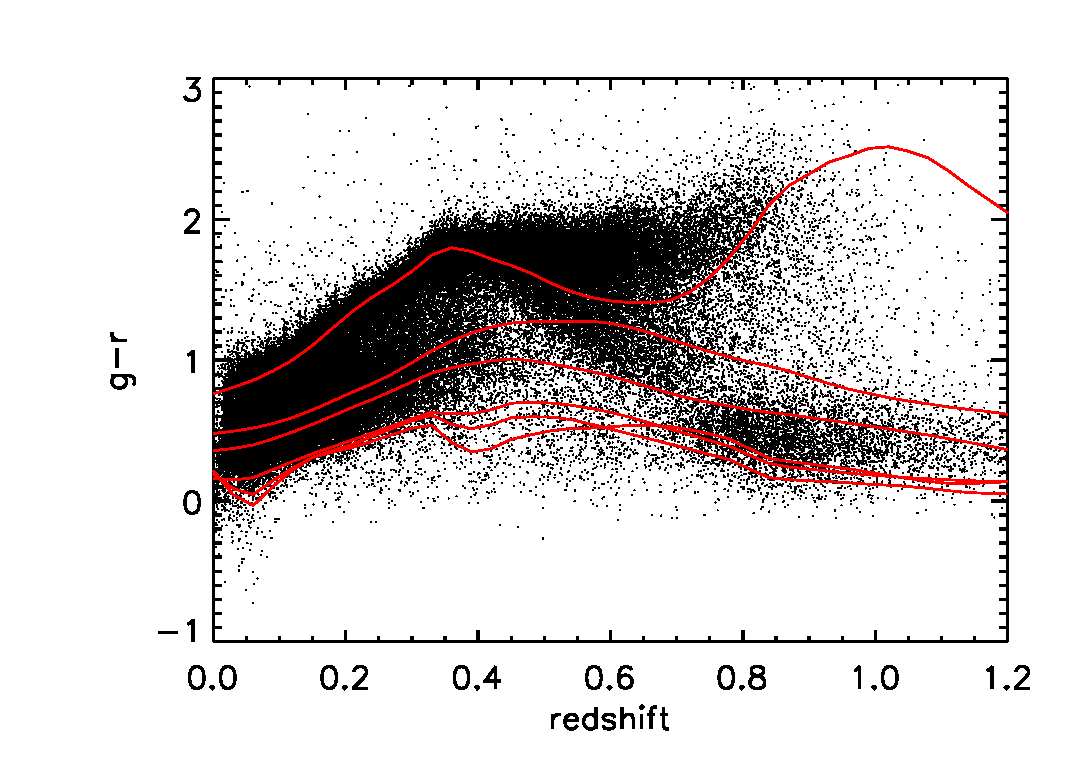
\includegraphics[width=0.5\textwidth]{figures/color_gr_z.eps}
	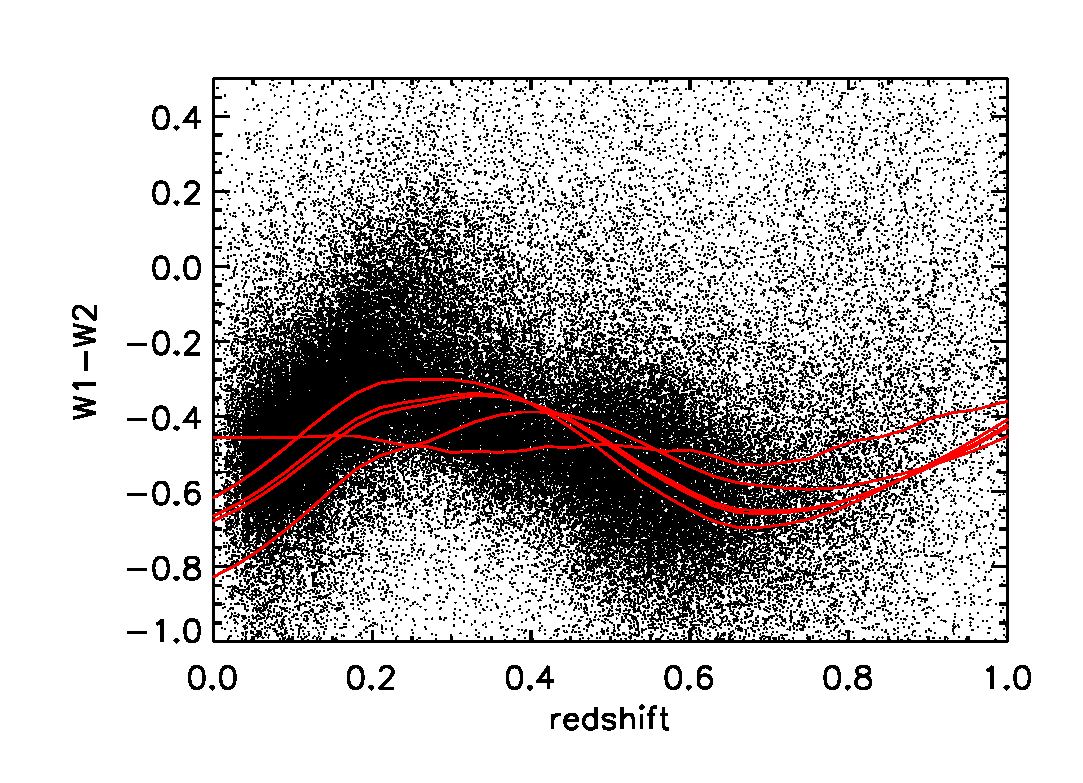
\includegraphics[width=0.5\textwidth]{figures/color_w1w2_z.eps}
	\caption{Color vs. spectroscopic redshift for the whole set of the photometric catalog sources (colored black) with available spectra. Colors of the six CWW+KIN templates as a function of redshift templates are plotted as red lines. These templates alone cover sufficient area on the plane and their linear combination returns reliable photometric redshift}
	\label{fig:color_z}
\end{figure*}

%Insert words from Konroy (ann.rev on photo_z)
The availability of near-IR filters helps improving the z phot accuracy beyond z $\approx$ 1.3, where the 4000A break goes out of the z 0 filter and the Lyman break is not yet detectable in the u - band. (from 1809.03373.pdf)

	comparison of the redshift with and without unWISE data (similar results)
And indeed near-IR bands W1 and W2 have negligible effect on the quality of the photometric redshift estimation within the redshift range of our data.
%\begin{figure*}[!ht]
%	\includegraphics[width=0.5\textwidth]{figures/photoz_7band.eps}
%	\includegraphics[width=0.5\textwidth]{figures/photoz_nowise.eps}
%	\caption{Photometric redshift vs. spectroscopic redshift. Sources in photometric catalog and SDSS DR14 spectroscopic catalogs are matched using 1$``$ matching radius}
%	\label{fig:photo_z}
%\end{figure*}

\subsection{FAST} 
	from Conroy review 2013:
	
	There has been some confusion in the literature regarding the importance of restframe NIR photometry for estimating stellar masses. First, as indicated in Figure 5, for smoothly varying SFHs, photometry at and redward of the V -band is sensitive to the same light- weighted age, and so redder bands do not provide stronger constraints on the mean stellar age. Taylor et al. (2011) analyzed mock galaxies and concluded that the addition of NIR data did not yield more accurate masses. Taylor et al. also found that different SPS models produced good agreement in derived properties when NIR data was excluded from their fits, but poor agreement when NIR was included. These authors also found much larger residuals in their SED fits when NIR data were included, suggesting that the models are still poorly calibrated in this regime. As discussed in Section 5.2, the NIR is at present probably most useful for constraining metallicities (within the context of a particular SPS model), and so NIR data may be useful in cases where there is a degeneracy between M / L and Z. In general however stellar mass estimates do not appear to be strongly improved with the addition of NIR data, at least with currently available models. Exceptions to this rule may be made for galaxies with very high dust opacities.
\section{Results}

\section{Discussion}

\section{Summary}


\acknowledgements


\bibliography{ms}{}
%\input{table3_allpar.tex}

\newpage
\centerline{ {\bf APPENDIX}}
\appendix

\section{Acknowledgments}
This publication makes use of data products from the Wide-field Infrared Survey Explorer, which is a joint project of the University of California, Los Angeles, and the Jet Propulsion Laboratory/California Institute of Technology, funded by the National Aeronautics and Space Administration. Part of our data processing and analysis were done using the HPC resources at the University of Missouri Bioinformatics Consortium (UMBC).

\end{document}
